%%%%% Don't Make Changes Below Here %%%%%
\documentclass{article}\usepackage[utf8]{inputenc}\usepackage[margin=0.4cm,top=0.4cm,bottom=0.4cm]{geometry}\usepackage[usenames,dvipsnames,svgnames,table]{xcolor}\usepackage{bm, multicol}\usepackage{calligra}\usepackage{tikz, listings}\usepackage{hyperref}\usetikzlibrary{matrix,fit,chains,calc,scopes}\usepackage{tcolorbox}\tcbuselibrary{skins}\tcbset{Baystyle/.style={sharp corners,enhanced,boxrule=6pt,colframe=orange,height=\textheight,width=\textwidth,borderline={8pt}{-11pt}{},}}\usepackage{amsmath,amssymb,amsthm,tikz,tkz-graph,color,chngpage,soul,hyperref,csquotes,graphicx,floatrow}\newcommand*{\QEDB}{\hfill\ensuremath{\square}}\newtheorem*{prop}{Proposition}\renewcommand{\theenumi}{\alph{enumi}}\usepackage[shortlabels]{enumitem}\usetikzlibrary{matrix,calc}\MakeOuterQuote{"}\newtheorem{theorem}{Theorem} \usetikzlibrary{shapes} \usepackage{lipsum}\usepackage{tabularx,ragged2e,booktabs,caption}\tcbuselibrary{breakable}\newenvironment{yframed}{\begin{tcolorbox}[breakable,colback=gray!3,title after break={\textit{\color{red}Solution (cont.)}},colbacktitle=gray!3, coltitle=black,titlerule=-1pt] }{\end{tcolorbox}}\newtcolorbox{mybox}{colback=black!15!white, colframe=white,arc=12pt}\newtcolorbox{myboxot}{colback=green!15!white, colframe=white,arc=12pt,width=110pt, height=27pt}\newtcbox{\mylib}{enhanced,boxrule=0pt,top=0mm,bottom=0mm,right=0mm,left=4mm,arc=4pt,boxsep=9pt,before upper={\vphantom{dlg}},colframe=green!50!black,coltext=green!25!black,colback=green!10!white,overlay={\begin{tcbclipinterior}\fill[green!75!blue!50!white] (frame.south west)rectangle node[text=white,font=\sffamily\bfseries\tiny,rotate=90] {Problem} ([xshift=4mm]frame.north west);\end{tcbclipinterior}}}\newtcbox{\mylibot}{enhanced,boxrule=0pt,top=0mm,bottom=0mm,right=0mm,arc=4pt,boxsep=9pt,before upper={\vphantom{dlg}},colframe=green!50!black,coltext=green!25!black,colback=green!10!white,overlay={\begin{tcbclipinterior}\fill[red!75!blue!50!white] (frame.south west)rectangle node[text=white,font=\sffamily\bfseries\tiny,rotate=90] {Other} ([xshift=4mm]frame.north west);\end{tcbclipinterior}}}
\def\Title{\begin{tcolorbox}[Baystyle,]{\begin{center}\vspace*{0.14\textheight}
{\rule{\textwidth}{1.6pt}\vspace*{-\baselineskip}\vspace*{2pt}}
\rule{\textwidth}{0.4pt}\\[0.2\baselineskip]{\fontsize{45}{45}\scshape CS 189: Introduction to Machine Learning \\[0.2\baselineskip] \calligra Spring 2018 \\[0.2\baselineskip]}
{\rule{\textwidth}{0.4pt}\vspace*{-\baselineskip}\vspace{3.2pt}}
\rule{\textwidth}{1.6pt}\\[\baselineskip]\vspace{0.05\textheight}{{\fontsize{45}{45}\scshape$\bullet$\\ {Homework 8}\\\vspace*{0.01\textheight} }{{\fontsize{18}{18}\scshape{Due on Friday, March 16th, 2018 at 10pm\\}}}\fontsize{45}{45}\scshape$\bullet$  \\}\vspace*{0.1\textheight}{\fontsize{12}{12}\calligra Solutions by\\}{\fontsize{28}{28}\scshape \Name \\}\vspace*{0.01\textheight}{\fontsize{12}{12}\scshape \SID} \\\vspace*{0.05\textheight}{\fontsize{12}{12}\calligra In collaboration with\\}\vspace*{0.01\textheight}{\fontsize{12}{12}\scshape \Collabs} \\\vspace*{0.05\textheight}\end{center}}\end{tcolorbox}\newgeometry{margin=0.75in}}\def\BeginSolution{\begin{yframed}\textbf{\color{red}Solution }}\def\EndSolution{\end{yframed}}\usepackage{algorithm}\usepackage[noend]{algpseudocode}\makeatletter\def\BState{\State\hskip-\ALG@thistlm}\makeatother\def\star{\bigstar}\usetikzlibrary{arrows}\usepackage[mathscr]{euscript}\usepackage[T1]{fontenc}\DeclareSymbolFont{rsfs}{U}{rsfs}{m}{n}\DeclareSymbolFontAlphabet{\mathscrsfs}{rsfs}\newcommand\tab[1][1cm]{\hspace*{#1}}\hypersetup{colorlinks=true,urlcolor=blue}\newtheorem{lemma}[theorem]{Lemma}\newcommand{\norm}[1]{\left\lVert#1\right\rVert}\def\vec{\mathbf}\def\y{\mathbf{y}}\def\X{\mathbf{X}}\def\R{\mathbb{R}}\def\x{\mathbf{x}}\def\w{\mathbf{w}}\def\T{^\top}\def\r{\mathbf{r}}\def\mat{\mathbf}\def\I{\mathbf{I}}\def\A{\mathbf{A}}\newcommand{\num}{n}\newcommand{\dims}{d}\def\real{\mathbb{R}}\def\ev{\mathbb{E}}\newcommand{\whatridge}{\widehat{w}_\lambda}\def\calN{\mathcal{N}}\newcommand{\hatwPCA}{\vec{\widehat{w}}_\text{{PCA}}}\newcommand{\hatyPCA}{\vec{\widehat{y}}_{\text{PCA}}}\newcommand{\hatwOLS}{\vec{\widehat{w}}_{\text{OLS}}}\newcommand{\hatwridge}{\vec{\widehat{w}}_{\text{ridge}}}\newcommand{\tildewridge}{\vec{\tilde{w}}_{\text{ridge}}}\newcommand{\hatyridge}{\vec{\hat{y}}_{\text{ridge}}}\def\diag{\operatorname{diag}}\newcommand*\circled[1]{\tikz[baseline=(char.base)]{\node[circle,fill=white!20,draw,inner sep=1pt,opacity=1,text opacity=0] (char) {#1};}}\newcommand\citem{\item[\circled{\Alph{enumi}}]}\def\hat{\widehat}
\def\lbreak{\vspace{4pt}

\noindent }
%%%%% Don't Make Changes Above Here %%%%%

%%%%% Template Begins Here %%%%%

\def\Name{Firstname Lastname}  % Your name
\def\SID{StudentID}  % Your student ID number
\def\Collabs{None} % Your collaborators here with a comma between each person's name. Write None if no collaborators. Don't leave blank.


\pagestyle{empty}
\begin{document}
\Title
\clearpage

%%%% Problem 1 Starts Here %%%%
\vspace{-2mm}\noindent\begin{mybox}{\begin{center}\textbf{\color{black}Problem 1: Getting Started}\end{center}}\end{mybox}\vspace{-2mm}
\vspace{10pt}
\noindent \textbf{Read through this page carefully.} You may typeset your homework in latex or submit neatly handwritten/scanned solutions. Please start each question on a new page. Deliverables:
\begin{enumerate}[1.]
\item Submit a PDF of your writeup, \textbf{with an appendix for your code}, to assignment on Gradescope, ``HW8 Write-Up''. If there are graphs, include those graphs in the correct sections. Do not simply reference your appendix.
\item If there is code, submit all code needed to reproduce your results, ``HW8 Code''.
\item If there is a test set, submit your test set evaluation results, ``HW8 Test Set''.
\end{enumerate}
After you've submitted your homework, watch out for the self-grade form.
\begin{enumerate}
\item Who else did you you work with on this homework? In case of course events, just describe the group. How did you work on this homework? Any comments about the homework?
\BeginSolution
%1a

\EndSolution
\item Please copy the following statement and sign next to it. We just want to make it \textit{extra} clear so that no one inadvertently cheats.

\textit{I certify that all solutions are entirely in my words and that I have not looked at another student's solutions. I have credited all external sources in this write up.}
\BeginSolution
%1b

\EndSolution
\end{enumerate}
%%%% Problem 1 Ends Here %%%%
\clearpage

%%%% Problem 2 Starts Here %%%%
\vspace{-2mm}\noindent\begin{mybox}{\begin{center}\textbf{\color{black}Problem 2: SGD on OLS}\end{center}}\end{mybox}\vspace{-2mm}
\vspace{10pt}
\noindent In this problem, we carefully walk through the key ingredients of a proof for SGD convergence for the specific example of a loss function which we are very familiar with: Ordinary Least Squares with positive definite matrix $\mat X^\top\mat X$.  In particular we show that in this case, even though gradient descent converges to the optimal solution of OLS, with small enough constant step-size, SGD is not guaranteed to do so! We then show that in contrast, when applying SGD with decaying step, as outlined in lecture, it does converge to the same optimum as gradient descent.
\lbreak
This phenomenon that constant step-size gets stuck and decaying step-sizes are the way out is analogous to common observations in practical machine learning problems, where decreasing the learning rate using heuristic learning rate schedules helps to decrease the training error.
\lbreak
Recall that the ordinary least squares problem can be written as: $$\min_{\vec w} f(\vec{w}) = \min_{\vec{w}} \frac{1}{2}\|\mat X\vec w - \vec y\|_2^2 = \min_{\vec{w}} = \frac{1}{2}\sum_{i=1}^n\left(\vec{x}_i^\top\vec{w} -\vec{y}_i\right)^2 = \min_{\vec w}\frac{1}{2}\sum_{i=1}^n f_i(\vec{w})$$ where $f-(\vec w) := \left(\vec{x}_i^\top\vec{w} -\vec{y}_i\right)^2$. Here $\vec{x}_i^\top$ is the $i$th row of matrix $\mat X$ and $f_i$ is the loss of the training example $i$. We implement SGD as follows: $$\vec{w}^{t+1} = \vec{w}^t - \alpha_t\nabla {f_{i}}_{t}\left(\vec{w}^t\right)$$ where $i_t$ is uniformly sampled from all samples $\{1,2,\ldots, n\}$ (and is  independently drawn for each iteration $t$). Let?s define the short hand $G_t = \nabla {f_i}_t\left(\vec{w}^t\right)$ to represent the random gradient at step $t$. We are interested in how $\vec{w}^t$ approaches the optimal solution $\vec{w}^*:=\arg\min_{\vec{w}\in\mathbb{R}^d} f(\vec{w})$. One way to characterize this is to monitor the squared distance of the iterate to the optimum, i.e. $\|\vec{w}^t - \vec{w}^*\|_2^2$. Throughout, we will assume that the following bound holds for the squared norm of
the stochastic gradient: \begin{align}\mathbb{E}\|G(\vec{w})\|_2^2\leqslant M_g^2\|\vec{w}-\vec{w}^*\|_2^2 + B^2\end{align} where $M_g$ and $B$ are are constants dependent on the model and loss function $f$. We will find concrete values of them later in this problem for specific examples. (Notice that in lecture we assumed $M_g$ to be zero, which is too restrictive even for the most basic least squares loss.)
\lbreak
\textbf{Problem outline: } Parts (a) - (c) help to derive a recursive formula of the form $$\mathbb{E}\|\vec{w}^{t+1}-\vec{w}^*\|_2^2\leqslant \gamma\mathbb{E}\|\vec{w}^t - \vec{w}^*\|_2^2 + \tilde{\gamma}$$ In part (d) we show that we achieve linear (also called geometric) convergence of $\vec{w}^t$ to the optimum $\vec{w}^*$ for SGD with constant step-size when $f(\vec{w}^*) = 0$. That means we can write $$\mathbb{E}\|\vec{w}^t - \vec{w}^*\|_2^2\leqslant \gamma^t\|\vec{w}^0-\vec{w}^*\|_2^2$$ for some $\gamma<1$. In part (e) we explore what happens with the iterates of SGD with constant step-size if instead $f(\vec{w}^*)>0$. In part (f) we visualize how the convergence bounds translate to actual training error decrease for OLS using SGD and GD.
\lbreak
The bonus parts (g) - (h) are for those students who "love math" according to the midterm preliminary questions, where you are asked to prove that SGD with decaying step-size converges at $\frac{1}{t}$ for "nice" functions using induction.
\begin{enumerate}
\item \textbf{Show that following relation between the $t+1$-step error and the $t$-step error: $$\|\vec{w}^{t+1} - \vec{w}^*\|_2^2 = \|\vec{w}^t - \vec{w}^*\|_2^2 - 2\alpha_t\langle G_t, \vec{w}^t-\vec{w}^*\rangle+\alpha_t^2\|G_t\|_2^2$$}
\BeginSolution
%2a

\EndSolution
\item \textit{Here we prove the key relation which underlies the success of stochastic gradient methods. This is where we use that stochastic gradients are unbiased!} Since we have stochastic gradients, we want to make guarantees in terms of expectations. For notational convenience let us define the short hand $\Delta_t:=\mathbb{E}_t\|\vec{w}^t-\vec{w}^*\|_2^2$, the \textit{average squared error},  where the expectation is taken over all the random indices drawn by the stochastic gradient method up to time $t$. We want to show a clean relation between $\Delta_t$ and $\Delta_{t+1}$ when the stochastic gradient satisfies (1).
\lbreak
Remind yourself which random indices $\vec{w}^t$ depends on and use the unbiasedness of the stochastic gradient to \textbf{show that \begin{align}\mathbb{E}\left[\langle G(\vec{w}^t), \vec{w}^t - \vec{w}^*\rangle\right] = \mathbb{E}\left[\langle\nabla f(\vec{w}^t), \vec{w}^t - \vec{w}^*\rangle\right]\end{align} Now use equality (2) and (a) to prove that \begin{align}\Delta_{t+1}\leqslant (1+\alpha_t^2M_g^2)\Delta_t - 2\alpha_t\cdot \mathbb{E}\left[\langle\nabla f(\vec{w}^t), \vec{w}^t - \vec{w}^*\rangle\right] + \alpha_t^2B^2\end{align}} \\ Hint 1: You may take the law of iterated expectation (also called tower property) as given, i.e. $$\mathbb{E}\left[\langle G(\vec{w}^t), \vec{w}^t - \vec{w}^*\rangle\right] = \mathbb{E}_{i_1,\ldots, i_{t-1}}\left[\mathbb{E}\left[\langle G(\vec{w}^t), \vec{w}^t - \vec{w}^*\rangle\mid i_1,\ldots,i_{t-1}\right]\right]$$ See Discussion for the derivation. 
\lbreak
Hint 2: Unbiased stochastic gradient means that $\mathbb{E}_{i_t}\left[\nabla f_{i_t}(\vec{w})\right] = \nabla f(\vec{w})$ for any $\vec{w}$ independent of the random index, where the expectation is with respect to the random index $i_t$ at time $t$. Refer to the Discussion for brief intro on conditional expectations.
\BeginSolution
%2b

\EndSolution
\item \textit{In this step we see that we need for our analysis that our loss function is "nice" (strongly convex to be precise), which holds for OLS when $\lambda_{\text{min}}\left(\mat X^\top \mat X\right)>0$. That is, all the guarantees for SGD we discuss in this problem only hold for such "nice" functions. In general, at least convexity is needed for any convergence proof.} \textbf{Using inequality (3), now show that $$\Delta_{t+1}\leqslant \left(1+\alpha t^2 M_g^2 - 2\alpha_t m\right)\Delta_t + \alpha_t^2 B^2$$ where we assume that the minimum eigenvalue of $\mat X^\top \mat X$ denoted by $m$ is positive, i.e. $$m:=\lambda_{\text{min}}\left(\mat X^\top \mat X\right)>0$$} \\ Hint: Use the fact that $\nabla f(\vec{w}^*)=\vec 0$, and hence $$\langle\nabla f(\vec{w}^t), \vec{w}-\vec{w}^*\rangle = \langle\nabla f(\vec{w}^t) - \nabla f(\vec{w}^*), \vec{w}-\vec{w}^*\rangle$$
\BeginSolution
%2c

\EndSolution
\item We now examine how close we can get to the optimal solution $\vec{w}^*$ using SGD with \textbf{constant step-size}, i.e. $\alpha_t = \alpha$ for all $t$ in two different scenarios. First, for this question we assume that $\mat X\vec{w}^* = \vec{y}$, or in other words, that the minimum loss is $0$. Show that inequality (1) holds with $B=0$ and $M_g=\max_{i}\|\vec{x}_i\|_2^4$ in this case. Find the optimum learning rate and show that $$\Delta_t\leqslant \left(1-\frac{m^2}{M_g^2}\right)^t\Delta_0$$ This means that with $B=0$ we have linear (geometric) convergence!
\lbreak
Hint: You may want to use that for any matrix $\mat A$ and vector $\vec{w}$ it holds that $$\|\mat A\vec{w}\|_2^2\leqslant \lambda_{\text{max}}(\mat A^\top \mat A)\|\vec{w}\|_2^2$$ and the same bound applies when taking the expectation on both sides.
\BeginSolution
%2d

\EndSolution
\item Instead of assuming that there exists a $\vec{w}^*$ that satisfies $\mat X\vec{w}^*=\vec{y}$ exactly, we now consider the case where $f(\vec{w}^*) = \frac{1}{2}\|\mat X\vec{w}^*-\vec{y}\|^2>0$. One can show that in this case $$\mathbb{E}\left[\|G(\vec{w})\|_2^2\right]\leqslant M_g^2\|\vec{w}-\vec{w}^*\|_2^2 + B^2$$ holds for some $M_g$ and $B$, where $M_g\neq 0$ and $B\neq 0$. Suppose that you are given the constants $M_g$ and $B$ and the step-size is still constant, i.e. $\alpha_t=\alpha$ for all $t$.
\lbreak We define the short hand notation $$\gamma:=1+\alpha^2 M_g^2 - 2\alpha m$$ and assume $\alpha$ is large enough such that $\gamma<1$. \textbf{Using part (c), prove that $$\Delta_t\leqslant \gamma^t\Delta_0 + \frac{\alpha B^2}{\alpha M_g^2 - 2m}$$} \\ We now want to interpret this bound. \textbf{Does it guarantee convergence $\vec{w}^t\to\vec{w}^*$ when $t$ goes to infinity? Explain.}
\lbreak
Hint: You may find the following inequality helpful: $$\sum_{t=1}^n \gamma^t\leqslant \frac{1}{1-\gamma}\quad\text{for }\gamma<1$$
\BeginSolution
%2e

\EndSolution
\item We now want use simulations to compare the first order methods for solving OLS for the cases in (d) and (e). In particular, we want to plot the estimation error $\|\vec{w}^t - \vec{w}^*\|_2$ against the gradient descent step in the following 3 scenarios:
\begin{itemize}
\item When there exists an exact solution $\mat X\vec{w}^* = \vec{y}$, plot the errors when you are using SGD and a constant learning rate.
\item When there does not exist an exact solution $\mat X\vec{w}^* = \vec{y}$, plot the errors when you are using SGD and a constant learning rate. Also plot the errors for GD and the same constant learning rate.
\item When there does not exist an exact solution $\mat X\vec{w}^* = \vec{y}$, plot the errors when you are using SGD and a decaying learning rate.
\end{itemize}
Using the attached starter code, \textbf{implement the gradient updates} in the function \texttt{sgd()}, while all the plotting functions are already there. \textbf{Show the 3 plots you obtain using the starter code. Report the average squared error computed in the starter code. What?s your conclusion?}
\BeginSolution
%2f

\EndSolution
\item (Bonus) \textbf{Prove that there is some constant $S$ and $k_0$ such that if the learning rate is decaying, the error $\Delta_k$ satisfies $$\Delta_k \leqslant \frac{S}{k+k_0}$$} \\ In this part, prove for the case of $M_g=0$ and $B\neq 0$.
\lbreak
Hint: Induction is your friend.
\BeginSolution
%2g

\EndSolution
\item (Bonus) \textbf{Prove that the same conclusion holds for the case of $M_g\neq 0$ and $B\neq 0$, for some different constants $M_g$ and $B$.}
\lbreak
Hint: This general case can be reduced to the case above.
\BeginSolution
%2h

\EndSolution
\end{enumerate}
%%%% Problem 2 Ends Here %%%%
\clearpage

%%%% Problem 3 Starts Here %%%%
\vspace{-2mm}\noindent\begin{mybox}{\begin{center}\textbf{\color{black}Problem 3: Gradient Descent Framework}\end{center}}\end{mybox}\vspace{-2mm}
\vspace{10pt}
\noindent In HW1, you modeled the classification of digit numbers of the MNIST dataset as a linear regression problem and solved it using its closed-form solution. In this homework, you will model it better by using classification models such as logistic regression and neural networks, and solve it using stochastic gradient descent. The goal of this problem is to show the power of modern machine learning frameworks such as TensorFlow and PyTorch, and how they can solve a wide range of problems. TensorFlow is the recommended framework in this homework and we also provide the starter kit in PyTorch.
\begin{enumerate}
\item The starter code contains an implementation of linear regression for the MNIST dataset to classify 10 digits. Let $\vec{x}_i$ be the feature vector and $\vec{y}_i$ be a one-hot vector encoding of its class, i.e. $y_{i,j}=1$ if and only if $i$th images is in class $j$ and $y_{i,j}=0$ if not. In order to use linear regression to solve a multi-class classification, we will use the \textit{one-vs-all} strategy here. In particular, for each $j$ we will fit a linear regression model $(\vec{w}_j, b_j)$ to minimize $\sum_i \left(\vec{w}_j^\top\vec{x}_i + b_j - y_{i,j}\right)_2^2$. Then for any image $\vec{x}$, the prediction of its class will be $\arg\max_j \left(\vec{w}_j^\top \vec{x}+b_j\right)$.
\lbreak
Read the implementation and run it with batch size equal to $50$, $100$, and $200$. \textbf{Attach the "epoch vs validation accuracy" plot. Report the running time for all the batch sizes. Explain the potential benefits and drawbacks of using small batch size, i.e., SGD vs GD.}
\BeginSolution
%3a

\EndSolution
\item \textbf{Implement the \texttt{train\_logistic\_function} to do the multi-class logistic regression using softmax function. Attach the plot of the "epoch vs validation accuracy" curve.} The loss function of the multi-class logistic regression is \begin{align}\ell = -\sum_{i=1}^n\log\left[\mathbf{{softmax}}\left(\mat W\vec{x}_i + b\right)^\top\vec{y}_i\right]\end{align} \\ where the softmax function $\mathbf{softmax}\,:\,\mathbb{R}^d\to\mathbb{R}^d$ is defined as \begin{align}\mathbf{softmax}(\vec{z})_j = \frac{\exp(z_j)}{\sum_k\exp(z_k)} = \frac{\exp(z_j - z')}{\sum_k\exp(z_k - z')}\end{align} \\ Here $z'=\max_j z_j$. The expression on the right is a numerical stable formula to compute the softma. You may NOT use any functions in \texttt{tf.nn.*}, \texttt{tf.losses.*}, and \texttt{torch.nn.*} for all parts of this problem.
\BeginSolution
%3b

\EndSolution
\item Copy your code from \texttt{train\_logistic} to \texttt{train\_nn} and add an additional \texttt{tanh} nonlinear layer to it. Your loss function should be something like  \begin{align}\ell = -\sum_{i=1}^n\log\left[\mathbf{{softmax}}\left(\mat W^{(2)}\mathbf{tanh}\left(\mat W^{(1)}\vec{x}_i\right) + \vec{b}\right)^\top\vec{y}_i\right]\end{align} \\ \textbf{Attach the plot of  of the "epoch vs validation accuracy" curve.} You have the freedom but \textbf{are NOT required to} choose the hyper-parameters to get the best performance.
\BeginSolution
%3c

\EndSolution
\item In our previous lecture, we learned how to solve the total least squares by doing the SVD decomposition. Now we will try to model the problem from the probabilistic perspective and solve it using stochastic gradient descent. Let the probabilistic model \begin{align}y_i - z_y = \vec{w}^\top (\vec{x}_i - \vec{z}_x)\end{align} where $\vec{x}_i$ and $y_i$ is the observed data, $y_i - z_y$ is $y_{\text{true}}$, $\vec{x}_i - z_\vec{z}$ is $x_{\text{true}}$, $z_y\sim\mathcal{N}(0,1)$, and $z_{\vec{x},j}\sim\mathcal{N}(0,1)$ for all $j$. \textbf{Prove that the log-likelihood for the model in Equation (7) is \begin{align}\sum_{i=1}^n\log P_\vec{w}(y_i\mid \vec{x}_i) = C - \frac{n}{2}\log\left(\|\vec{w}\|_2^2 + 1\right) - \frac{1}{2\left(\|\vec{w}\|_2^2 + 1\right)}\sum_{i=1}^n\left(y_i - \vec{w}^\top\vec{x}_i\right)^2\end{align}} \\ where $n$ is the number of samples, and $C$ is a constant that is not related to $\vec w$, $y$, and $x$. \textit{Note that the maximum likelihood estimation of this probabilistic model is not the same as the SVD solution of TLS as we did in lecture.}
\BeginSolution
%3d

\EndSolution
\item \textbf{Implement the stochastic gradient descent to find the MLE for the model above.} In the starter code, we generate some data for you and you will need to recover $\vec w$ using the observed data. \textbf{Report the error} $\|w^* - w_{\text{true}}\|_2^2$ where $w^*$ is the one that you recover. Try to play with hyper-parameters such as the batch size and the learning rate. \textbf{Is the solution of SGD sensitive to its hyper-parameters in this problem?}
\BeginSolution
%3e

\EndSolution
\end{enumerate}
%%%% Problem 3 Ends Here %%%%
\clearpage

%%%% Problem 4 Starts Here %%%%
\vspace{-2mm}\noindent\begin{mybox}{\begin{center}\textbf{\color{black}[BONUS] Problem 4: Genome-Wide Association Study}\end{center}}\end{mybox}\vspace{-2mm}
\vspace{10pt}
\noindent \textbf{All the following text is present in the accompanying Jupyter notebook, but the notebook has additional explanations and accompanying figures and code. We recommend you do not read this pdf, but go directly to the Jupyter notebook. This pdf was included for quick reference.}
\lbreak
\underline{Overall goal}: This real world problem is one in computational biology which uses many of the techniques and concepts you have been introduced to, all together, in particular, linear regression, PCA, non-iid noise, diagonalizing multivariate Gaussian covariance matrices, and bias-variance trade-off. We will also tangentially introduce you to concepts of statistical testing. \textbf{This homework problem is effectively a demo in that we will ask you to execute code and answer questions about what you observe. You are not required to code anything at all.}
\lbreak
\underline{Setup and problem statement}: Given a set of people for whom genetics (DNA) has been measured, and also a corresponding trait for each person, such as blood pressure, or "is-a-smoker", one can use data-driven methods to deduce which genetic effects are likely responsible for the trait. We have collected blood from $n$ individuals who either smoke ($y_i = 1$) or do not smoke ($y_i = 0$). Their blood samples have been sequenced at m positions along the genome, yielding the feature matrix $\mat X\in \mathbb{R}^{n\times m}$, composed of the genetic variants (which take on values $0$, $1$, or $2$). Specifically, $\mat X_{i,j}$ is a numeric encoding of the DNA for the $i$ \textsuperscript{th} person at genetic feature $j$.\footnote{Technically, the entries of the matrix correspond to having zero, one or two mutant versions of the DNA, but we will treat them as real-valued in this problem.} We want to deduce which of the $m$ genetic features are associated with smoking, by considering one at a time. \textit{In the data we give you, it will turn out that there is no true signal in the data; however, we will see that without careful modeling, we would erroneously conclude that the data were full of signal.}
\lbreak
\underline{Overall modeling approach}: The basic idea will be to "test" one genetic feature at a time and assign a score (a $p$-value) indicating our level of belief that it is associated with the trait. We will start with a simple linear regression model, and then build increasingly more correct linear predictive models. The three models we will use are (1) linear regression, (2) linear regression with PCA features, (3) linear regression with all genetic variants as features. The first model is naive, because it assumes the individuals are iid. The fundamental modeling challenges with these kinds of analyses is that the individuals in the study are not typically not iid, owing to differences in race and family-relatedness (e.g., sisters, brothers, patients, grandparents in the data set), which violate the iid assumption. Left un-modeled, such structure creates misleading results, yielding signal where none exists. Luckily, as we shall see, one can visualize these modeling issues via quantile-quantile plots, which will soon be briefly introduced.
\lbreak
\underline{How to test each variant}: Herein we provide a minimal exposition to allow you to do the homework To estimate how implicated each genetic feature is we will use a score, in the form of a $p$-value. One can think of the $p$-value as a proxy for how informative the genetic feature is for prediction of the trait (e.g. "is smoker"). More precisely, to get the $p$-value for the $j$\textsuperscript{th} genetic feature, we first include it in the model (for a given model class, such as linear regression) and compute the maximum likelihood, $LL_j$ (this is our alternative hypothesis). Then we repeat this process, but having removed the genetic feature of interest from the model, yielding $LL_{-j}$ (this is our null hypothesis). To be clear, the null hypothesis will have none of the m genetic variants that are being tested. You can refer to the Jupyter notebook for a brief explanation of hypothesis testing. The $p$-value is then a simple monotonic decreasing function of the difference in these two likelihoods, \texttt{diff\_ll} $= LL{j} - LL_{-j}$-one that we will give you. $p$-values lie in $[0, 1]$ and the smaller the $p$-value, the larger the difference in the likelihoods, and the more evidence that the genetic marker is associated with the trait (assuming the model is correct).
\begin{enumerate}
\item To diagnose if something is amiss in our genetic analyses, we will make use of the following: (1) we assume that if any genetic signal is present, it is restricted to a small fraction of the genetic features, (2) $p$-values corresponding to no signal in the data are distributed as $p\sim \operatorname{Unif}[0, 1]$. Combining these two assumptions, we will assume that $p$-values arising from a valid model should largely be drawn from $\operatorname{Unif}[0, 1]$, and also that large deviations suggest that our model is incorrect. Quantile-quantile plots let us visualize if we have deviations or not. Quantile-quantile plots are a way to compare two probability distributions by comparing their quantile values (e.g. how does the smallest $p$-value in each distribution compare, and then the second smallest, etc.). In the quantile-quantile plot, you will see $m$ points, one for each genetic marker. The $x$-coordinate of each point corresponds to the theoretical quantile we would expect to see if the distribution was in fact a $\operatorname{Unif}[0, 1]$ and the $y$-coordinate corresponds to the observed value of the quantile. An example is shown in Figure 1~\ref{fig:qqplot}, where the line on the diagonal results from an analysis where the model is correct, and hence the theoretical and empirical p-value quantiles match, while the other line, which deviates from the diagonal, indicates that we have likely made a modeling error. If there are genetic signals in the data, these would simply emerge as a handful of outlier points from the diagonal (not shown).
\begin{figure}[h!]    \begin{center}    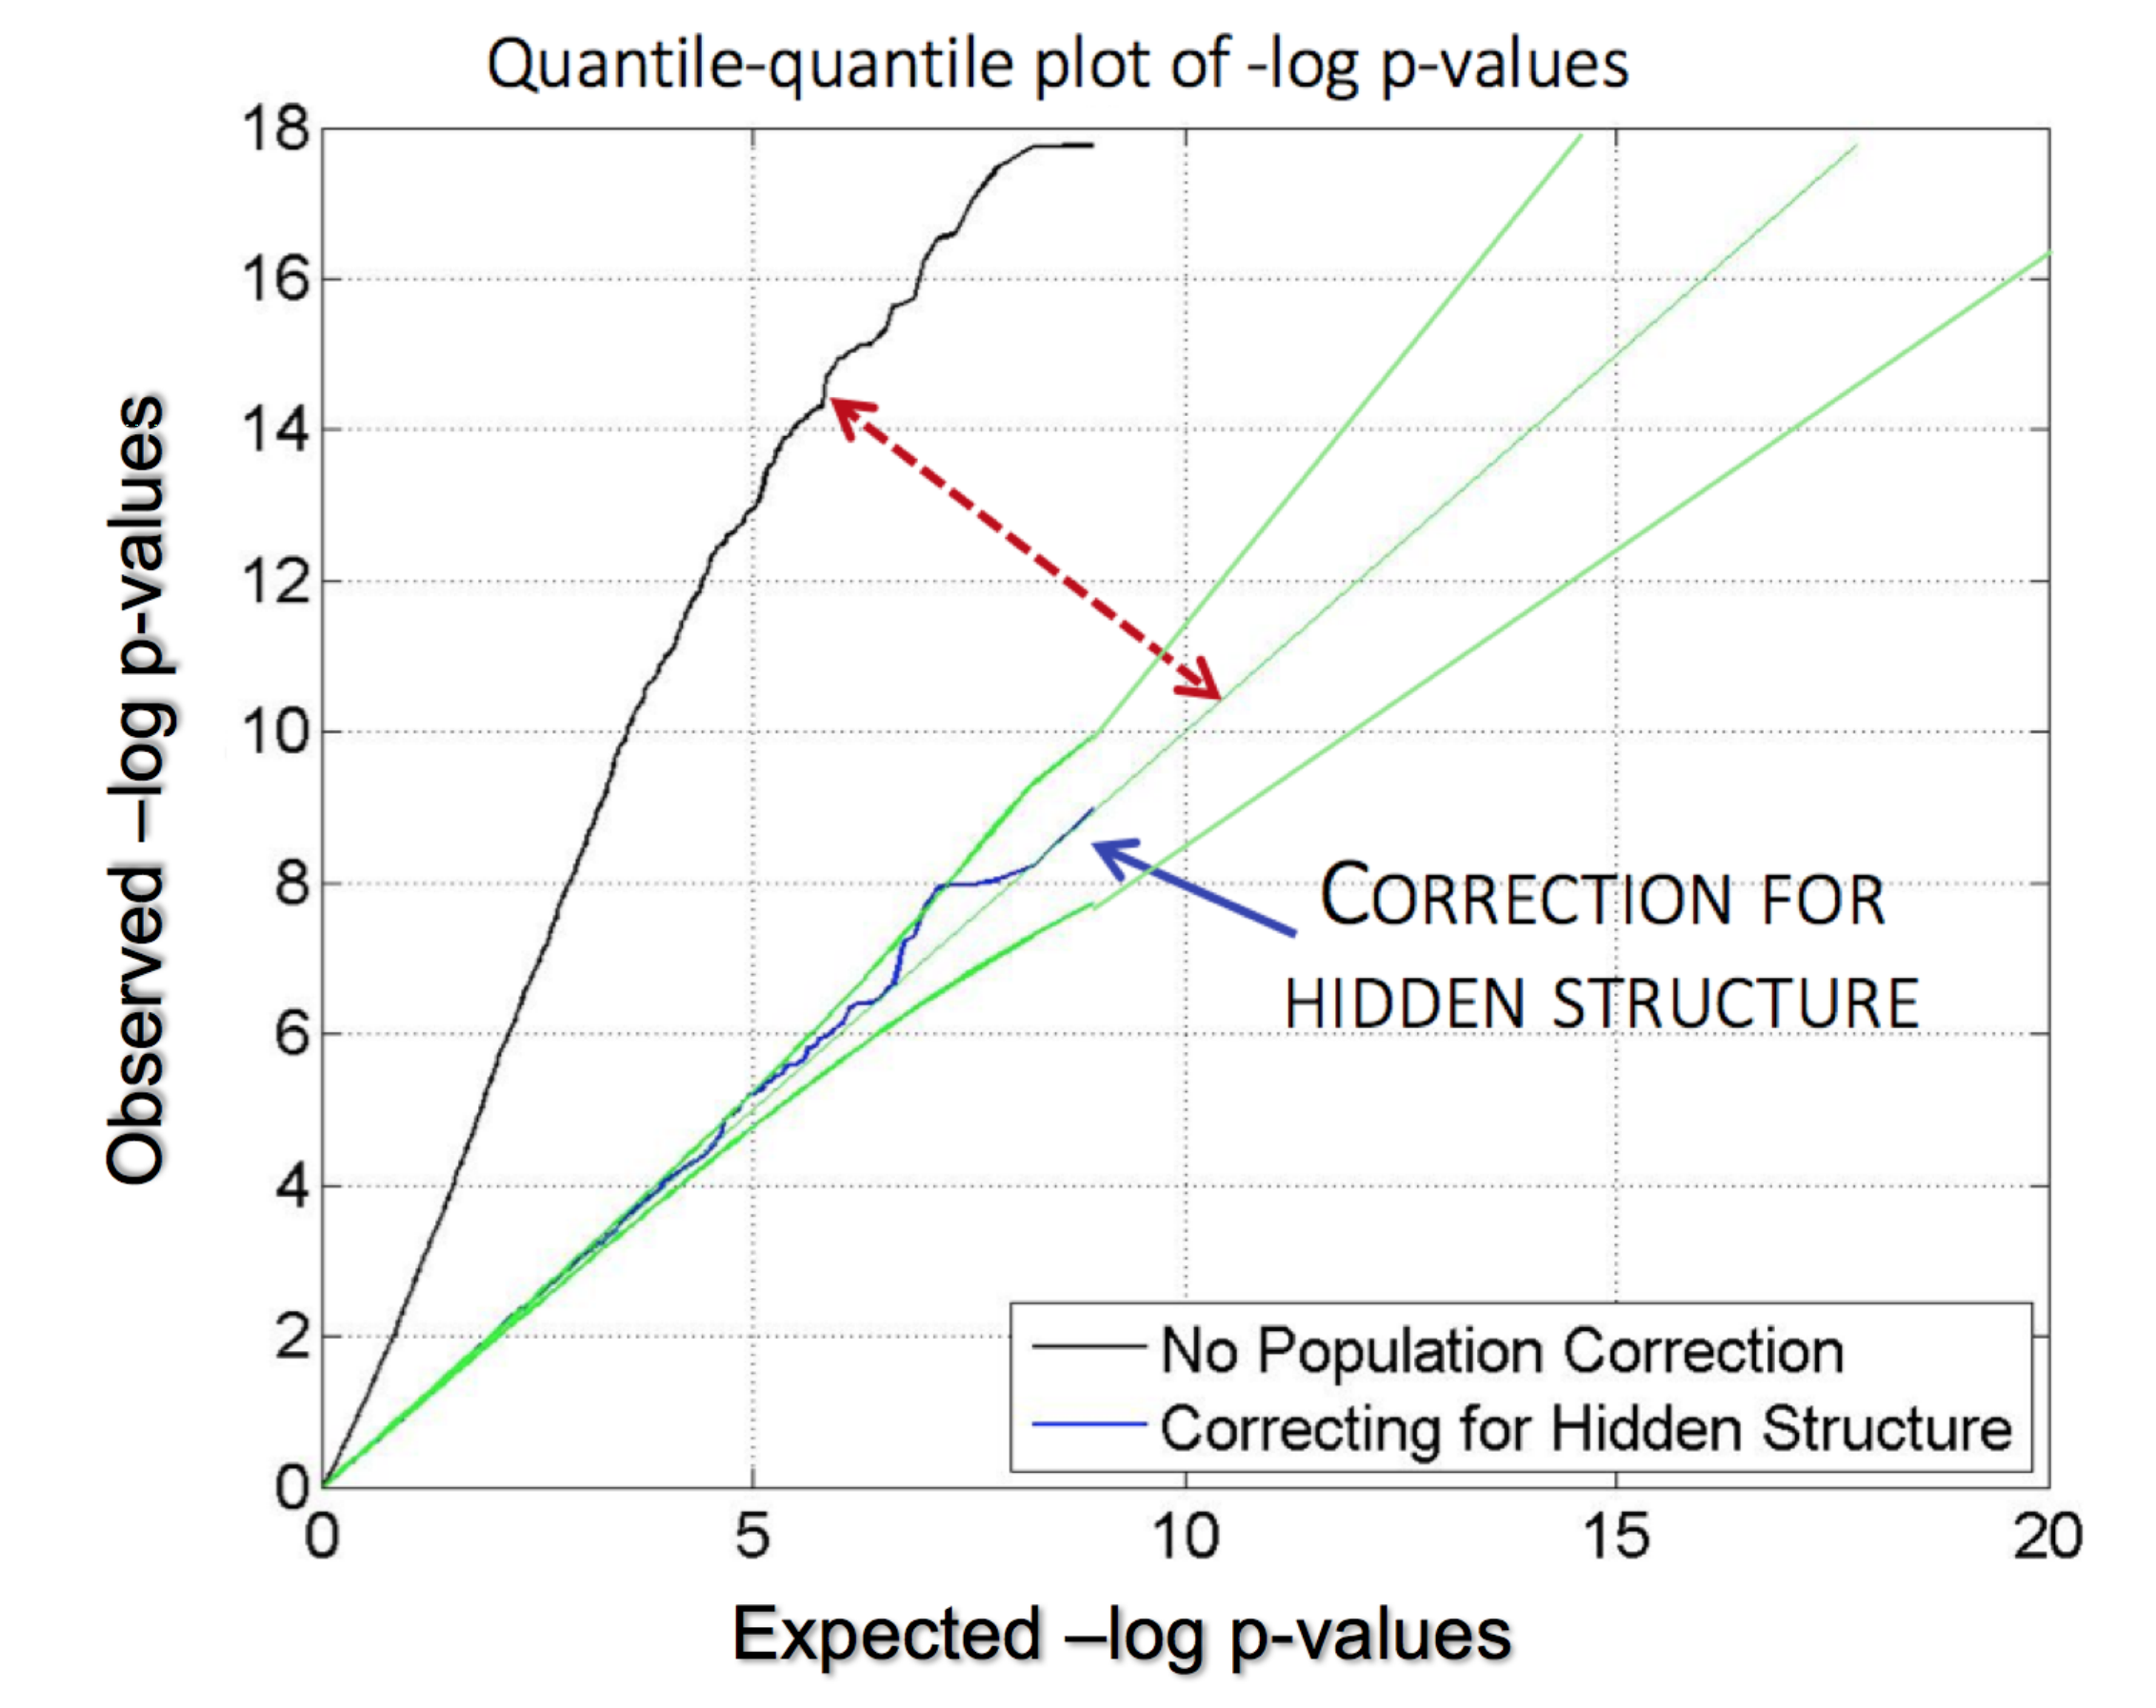
\includegraphics[scale=.3]{qqplot}    \caption{ Example of quantile-quantile plot that shows large deviation from expectation.}    \label{fig:qqplot}\end{center}\end{figure}
\lbreak Before we dive into developing our models, we need to be able to understand whether the $p$-values we get back from our hypothesis tests look like m random draws from a $\operatorname{Unif}[0, 1]$.
\lbreak
\textbf{Use the qqplot function to make a qq-plot for each of the $3$ distributions provided below and explain your findings. What should we observe in our qq-plot if our empirical distribution looks more and more similar to a $\operatorname{Unif}[0, 1]$?} Note that we use two kinds of qq-plots: one in $p$-value space and one negative $\log$ $p$-value space. The former is for intuition, while the latter is for higher resolution. The green lines in the negative $\log$ $p$-value qq-plots indicate the error bars.
\BeginSolution
%4a

\EndSolution
\item We will use linear models in the genetic marker we are testing. In particular, when testing
the $j$\textsuperscript{th} genetic feature, we have that the trait, $y$, is a linear function of the genetic variant, i.e. $\vec{y} = \vec{x}_j w_i + \vec{w}_0 + \bm{\epsilon}$ where $\epsilon_i$ is random noise distributed as $\mathcal{N}(0,\sigma^2)$, $w_1\in\mathbb{R}^1$, $\vec{w}_0\in\mathbb{R}^{n\times 1}$ is a constant vector, and $\vec{x}_j$ is the $j$\textsuperscript{th} column of $\mat X$, representing data for the $j$\textsuperscript{th} genetic variant. To simplify matters, we will add a column of ones to the right end of $\vec{x}_j$ and rewrite the regression as $\vec{y} = [\vec{x}_j, \vec{1}]\vec{w}+\bm{\epsilon}$ where $[\vec{x}_j, \vec{1}]$ is the $j$\textsuperscript{th} column of $\mat X$ with a vector of ones appended to the end and $\vec{w}\in\mathbb{R}^{2\times 1}$. The model without any genetic information, $\vec{y} = \vec{1}w + \bm{\epsilon}$ is referred to as the \textit{null model} in the parlance of statistical testing the \textit{alternative model}, which includes the information we are testing (one genetic marker) is $\vec{y} = [\vec{x}_j, \vec{1}]\vec{w}+\bm{\epsilon}$ where $\vec{x}_j$ is the $j$\textsuperscript{th} column of $\mat X$, i.e. the data using only the $j$\textsuperscript{th} genetic variant as a feature. \textbf{Plot the quantile quantile plot of $p$-values using linear regression as just describe, a so-called naive approach, by running the function \texttt{naive\_model}. From the plot, what do you conclude about the suitability of linear regression for this problem?}
\BeginSolution
%4b

\EndSolution
\item From the quantile-quantile plot in the previous part, it appears that the model is picking up on more association than theoretically expected. The reason for this is owing to the assumption of iid noise being correct. In particular, this data set contains individuals from different racial backgrounds, and also has clusters of individuals from extended families (e.g. grandparents, parents, siblings). This means that their genetics are not iid, and hence linear regression yields spurious results-all the genetic features seem to be implicated in the trait. Thus we need to modify our noise assumptions by somehow accounting for the hidden structure in the data set. The main idea is that when testing one genetic feature, all the other genetic features, jointly, are a proxy to the racial and family background. If we could include them in our model, we could correct the problem. \textbf{Ideally we would like to use all the genetic features in the linear regression model, however this is not a good idea. Why not?} Hint: There are roughly $1300$ individuals and $7500$ genetic variants. A written, English answer is sufficient.
\lbreak
So instead of using all genetic features, we will try using PCA to reduce the number of genetic features. As we saw in class, PCA on a genetic similarity matrix can capture geography, which correlates to race, quite well. So instead of adding all the genetic features, we will instead use only three features\footnote{One needs to choose this number, but we have done so for you} $\mat{X}_{\text{proj}}$, which are the $\mat X$ projected onto the top $3$ principal components of $\mat X$. Consequently, the updated null model is $\vec{y} = \mat{X}_{\text{proj}}\vec{w}_{\text{proj}} + \bm{\epsilon}$ where $\vec{w}_{\text{proj}}\in\mathbb{R}^{3\times 1}$, while the alternative model is $\vec{y} = [\vec{x}_j, \mat{X}_{\text{proj}}, \vec{1}]\vec{w}+\bm{\epsilon}$ where $\vec{w}\in\mathbb{R}^{5\times 1}$ for genetic variant $j$. \textbf{Plot the quantile-quantile plot from obtaining p-values with this PCA linear regression approach by running the function \texttt{pca\_corrected\_model}. How does this plot compare to the first plot? What does this tell you about this model compared to the previous model?}
\BeginSolution
%4c

\EndSolution
\item PCA got us part of the way there. However, PCA truncates the eigen-spectrum; if the tail-end of that spectrum is important, as it is for family-relatedness, then it will not fully correct for our problem. So we want a method which (a) is well-behaved in terms of number of parameters that need to be estimated, and (b) includes all of the information we need. So rather than adding the projections as features, we use an modeling approach called linear mixed models which effectively adjust the iid noise in the gaussian by the pairwise genetic similarity of all the individuals. That is, we set $\Sigma$ in $\vec{y}\sim\mathcal{N}\left(y\mid [\vec{x}_j,1]\vec{w},\mat{I}\sigma^2 + \mat X\mat X^\top\sigma_k^2\right)$.
\lbreak
Specifically, $\vec{y} = [\vec{x}_j, 1]\vec{w} + \vec{z} + \bm{\epsilon}$ where $\vec{z}\sim \mathcal{N}(0,\sigma_k^2\mat K)$ where $\mat K = \mat X\mat X^\top$, $\sigma_k$, $\vec{w}\in\mathbb{R}^{m\times 1}$ and $\sigma$ are parameters we want to estimate. Notice that $\vec{y}\sim\mathcal{N}\left([\vec{x}_j, 1]\vec{w},\sigma^2\mat I + \sigma_k^2\mat K\right)$.  Evaluation of the likelihood is thus on the order of $\mathcal{O}(n^3)$ from the required matrix inverse and determinant of $\sigma^2\mat I + \sigma_k^2\mat K$. To test $m$ genetic variants, the time complexity becomes $\mathcal{O}(mn^3)$, which is extremely slow for large datasets. \textbf{Given the eigen-decomposition $\mat K = \mat U \mat D\mat U^\top$, how
can we make this faster if we have to test thousands of genetic feature? Would this be computationally more efficient if you only have one genetic feature to test?}
\lbreak
\textbf{Finally, make the quantile-quantile plot for this last model by running the function \texttt{lmm}. What can we conclude about this model relative to the other two models?}
\lbreak
HINT: Since the manipulations needed for $\sigma^2\mat I + \sigma_k^2\mat K$ is the bottleneck here, we would like a transformation which makes this covariance of the multi-variate gaussian be a diagonal matrix.
\BeginSolution
%4d

\EndSolution
\end{enumerate}
%%%% Problem 4 Ends Here %%%%
\clearpage

%%%% Problem 5 Starts Here %%%%
\vspace{-2mm}\noindent\begin{mybox}{\begin{center}\textbf{\color{black}Problem 5: Your Own Question}\end{center}}\end{mybox}\vspace{-2mm}
\vspace{10pt}
\noindent \textbf{Write your own question, and provide a thorough solution.}
\vspace{3pt}

\noindent Writing your own problems is a very important way to really learn the material. The famous ``Bloom's Taxonomy'' that lists the levels of learning is: Remember, Understand, Apply, Analyze, Evaluate, and Create. Using what you know to create is the top-level. We rarely ask you any HW questions about the lowest level of straight-up remembering, expecting you to be able to do that yourself. (e.g. make yourself flashcards) But we don't want the same to be true about the highest level.
\vspace{3pt}

\noindent As a practical matter, having some practice at trying to create problems helps you study for exams much better than simply counting on solving existing practice problems. This is because thinking about how to create an interesting problem forces you to really look at the material from the perspective of those who are going to create the exams. 
\vspace{3pt}

\noindent Besides, this is fun. If you want to make a boring problem, go ahead. That is your prerogative. But it is more fun to really engage with the material, discover something interesting, and then come up with a problem that walks others down a journey that lets them share your discovery. You don't have to achieve this every week. But unless you try every week, it probably won't happen ever. 
\BeginSolution
%5

\EndSolution
%%%% Problem 5 Ends Here %%%%
\clearpage

%%%% Code Appendix Starts Here %%%%
\vspace{-2mm}\noindent\begin{mybox}{\begin{center}\textbf{\color{black}Code Appendix}\end{center}}\end{mybox}\vspace{-2mm}
\begin{itemize}
\item \texttt{starter\_P1\_SGDtheory.ipynb}
\BeginSolution
% Paste Code Between Verbatim
% starter_P1_SGDtheory.ipynb
\begin{verbatim}

\end{verbatim}
\EndSolution
\item \texttt{starter\_P3\_classification/classification\_pytorch.py}
\BeginSolution
% Paste Code Between Verbatim
% starter_P3_ classification/classification_pytorch.py
\begin{verbatim}

\end{verbatim}
\EndSolution
\item \texttt{starter\_P3\_classification/classification\_tensorflow.py}
\BeginSolution
% Paste Code Between Verbatim
% starter_P3_ classification/classification_tensorflow.py
\begin{verbatim}

\end{verbatim}
\EndSolution
\item \texttt{starter\_P3\_classification/tls\_pytorch.py}
\BeginSolution
% Paste Code Between Verbatim
% starter_P3_ classification/tls_pytorch.py
\begin{verbatim}

\end{verbatim}
\EndSolution
\item \texttt{starter\_P3\_classification/tls\_tensorflow.py}
\BeginSolution
% Paste Code Between Verbatim
% starter_P3_ classification/tls_tensorflow.py
\begin{verbatim}

\end{verbatim}
\EndSolution
\item \texttt{code\_P4\_genome/gwas problem.ipynb}
\BeginSolution
% Paste Code Between Verbatim
% code_P4_genome/gwas problem.ipynb
\begin{verbatim}

\end{verbatim}
\EndSolution
\end{itemize}
%%%% Code Appendix Ends Here %%%%

\end{document}
%%%%% Template Ends Here %%%%%